\documentclass[10pt, xcolor=dvipsnames]{beamer}
%\documentclass[10pt, xcolor=dvipsnames,notes=only]{beamer}
%\mode<presentation>
%{
\usetheme{Goettingen}
%\setbeamercovered{transparent}
%} 
\usefonttheme{professionalfonts}
%\usecolortheme{beaver}

\usepackage{setspace}
\usepackage[english]{babel}
\usepackage[latin1]{inputenc}
\usepackage{times}
\usepackage[T1]{fontenc}
\usepackage{color}
\usepackage{graphicx}
\usepackage{amssymb}
\usepackage{amsthm}
\usepackage{bm}
\usepackage{rotating}
\usepackage{ccaption}
\usepackage{booktabs}
\usepackage{lscape}
\usepackage{colortbl}
\usepackage{arydshln}
\usepackage{tabularx}
\usepackage{graphics}
\usepackage{epstopdf}

\setbeamertemplate{navigation symbols}{}
\setbeamertemplate{items}[balls]

\newenvironment{changemargin}[2]{%
  \begin{list}{}{%
    \setlength{\topsep}{0pt}%
    \setlength{\leftmargin}{#1}%
    \setlength{\rightmargin}{#2}%
    \setlength{\listparindent}{\parindent}%
    \setlength{\itemindent}{\parindent}%
    \setlength{\parsep}{\parskip}%
  }%
  \item[]}{\end{list}}

\setbeamercolor{block title}{fg=white, bg=teal}
\setbeamercolor{block body}{bg=teal!25}

\author[]{Chad Jones and Dietrich Vollrath}
\institute[Intro Growth]{Introduction to Economic Growth}
\date[]{}


\title[Population]{Population and the origin of sustatined growth}


\begin{document}
\maketitle

\section{The Malthusian economy}
\begin{frame}{Historical take-off}
\begin{center}
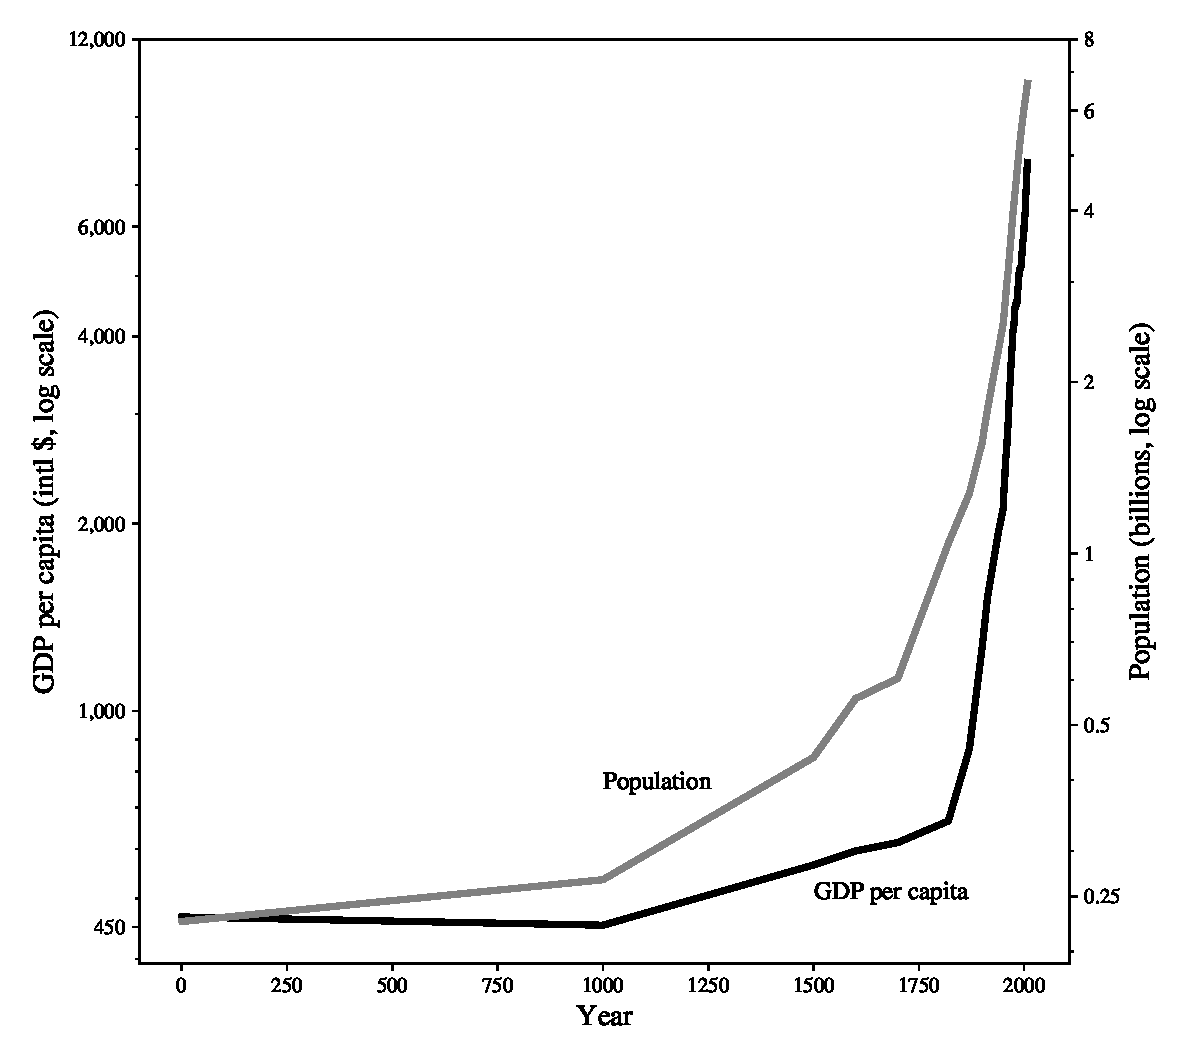
\includegraphics[height=3in]{../Figures/fig-ch9-fig1.eps}
\end{center}
\end{frame}

\begin{frame}{A Malthusian economy}
Malthus speculated on how fixed/limited resources influenced population growth and living standards. Let production be
\begin{equation}
	Y_t = X^{\beta}\left(A_t^{\beta/(1-\beta)} L_t\right)^{1-\beta} \nonumber
\end{equation}
where $X$ is the amount of the fixed resource. $\beta$ is how important that is in production. $L_t$ is population.
\vspace{.25in}\noindent
$A_t$ is productivity. The exponents are for simplification.
\end{frame}

\begin{frame}{Living standards}
In per-capita terms this is
\begin{equation}
	y_t = \left(\frac{A_tX}{L_t}\right)^{\beta}. \label{EQ_y_malthus}
\end{equation}
Living standards depend
\begin{itemize}
	\item positively on $A_t$
	\item positively on $X_t$
	\item \textit{negatively} on $L_t$
\end{itemize}
\end{frame}

\begin{frame}{Endogenous population growth}
For Malthus, population growth isn't given, it depends on $y_t$
\begin{equation}
	g_L = \nu (y_t - \overline{c}) \nonumber
\end{equation}
where $\nu$ is scaling and $\overline{c}$ is a ``subsistence'' level of consumption:
\begin{itemize}
	\item If $y_t > \overline{c}$, population growth is positive. Lower mortality, higher family formation and fertility.
	\item If $y_t < \overline{c}$, population growth is negative. High mortality, limited family formation and fertility.
	\item As $y_t$ goes up, so does $g_L$
\end{itemize}
\end{frame}

\begin{frame}{Dynamics of population}
Plug in what we know about $y_t$ and you have
\begin{equation}
	g_L = \nu \left(\frac{A_tX}{L_t}\right)^{\beta} - \nu \overline{c}. \label{EQ_gL_malthus}
\end{equation}
\begin{itemize}
	\item This is a dynamic system telling us that $g_L$ relates to a ratio $AX/L$. 
	\item $g_L$ is negatively related to $L$. More people, lower living standards, lower population growth.
	\item This is similar analysis to Solow/Romer and other dynamic models.
\end{itemize}
\end{frame}

\begin{frame}{Malthusian dynamics}
\begin{center}
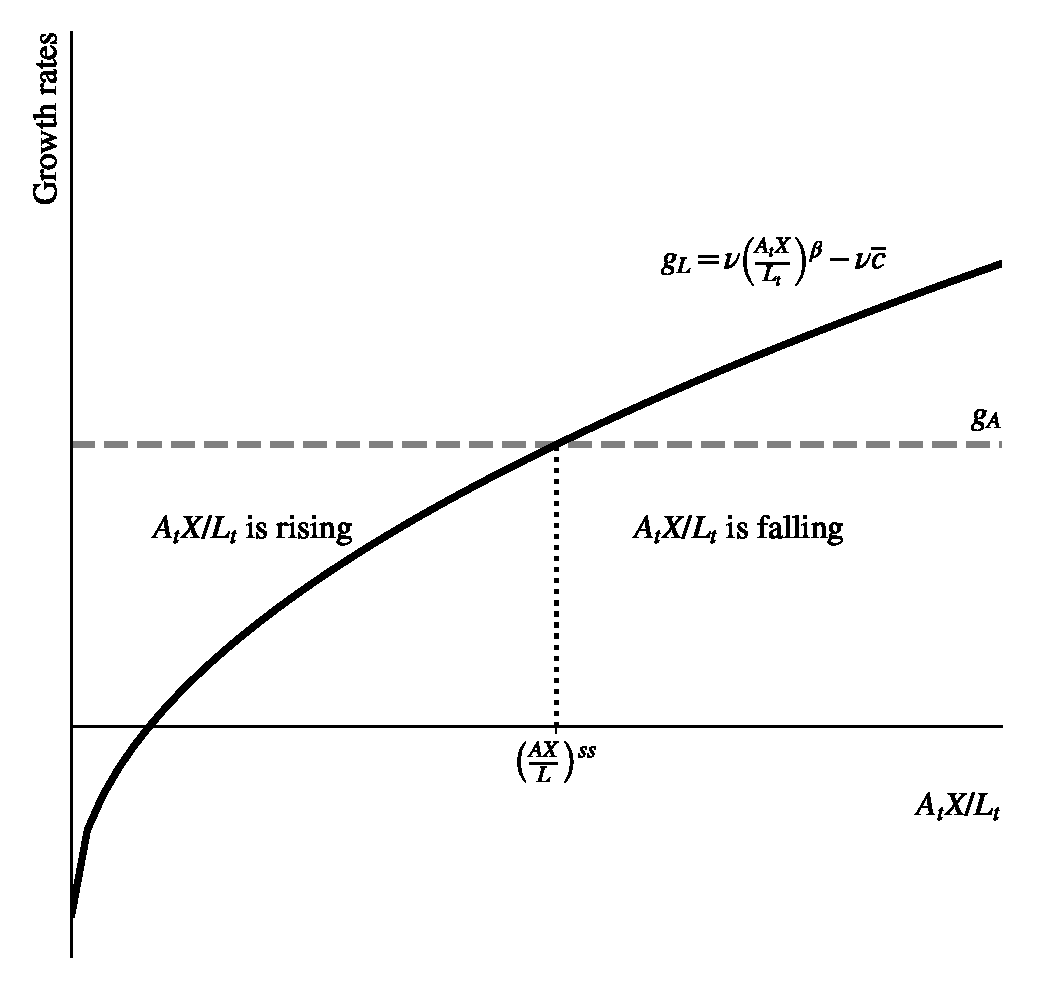
\includegraphics[height=3in]{../Figures/fig-ch9-fig2.eps}
\end{center}
\end{frame}

\begin{frame}{Malthusian steady state}
In the steady state it's the case that $g_L^{ss} = g_A$. From production function we have
\begin{equation}
	g_y = \beta(g_A - g_L). \label{EQ_gy_malthus}
\end{equation}
so in steady state it must be that $g_y^{ss} = 0$. In the Malthusian world living standards don't grow.
\vspace{.25in}\noindent
If $g_y = 0$, the it must be the case that
\begin{equation}
	y^{ss} = \frac{g_A}{\nu} + \overline{c}. \label{EQ_yss_malthus}
\end{equation}
as this ensures $g_L = g_A$. 
\end{frame}

\begin{frame}{Malthusian steady state}
Given
\begin{equation}
	y^{ss} = \frac{g_A}{\nu} + \overline{c}. \label{EQ_yss_malthus}
\end{equation}
\begin{itemize}
	\item Living standards are \textit{higher} than the subsistence level $\overline{c}$
	\item How much higher depends on $g_A$. Productivity growth allows you to stay ahead.
	\item $\overline{c}$ isn't a biological minimum, it depends on culture/society as much as biology
	\item Malthusian economies can be relatively well-off, but stagnant
\end{itemize}
\end{frame}

\begin{frame}{Malthusian effects}
Malthus is kind of depressing. A substantial loss of population:
\begin{itemize}
	\item Raises living standards for the remaining people
	\item Who then start to have more children in response
	\item Which lowers living standards
	\item Until living standards are back at the level before the shock to population
\end{itemize}
This happened historically with the Black Death. 
\end{frame}

\section{Endogenous technology}
\begin{frame}{Escaping Malthus}
The world economy does not appear to be in a Malthusian situation, we have sustained economic growth. Two important elements to escape:
\begin{itemize}
	\item Innovation/technology accelerated
	\item Population growth changed it's relationship to living standards
\end{itemize}
\end{frame}

\begin{frame}{Endogenize innovation}
Our general structure was
\begin{equation}
	g_A = \theta \frac{(s_R L_t)^{\lambda}}{A_t^{1-\phi}}, \label{EQ_ga_malthus}
\end{equation}
but here let
\begin{itemize}
	\item $s_R = 1$, or everyone could potentially innovate
	\item $\lambda = 1$
	\item $\phi = 1$. We know this is wrong in modern world, but could be applicable before that
\end{itemize}
which gives us
\begin{equation}
	g_A = \theta L_t
\end{equation}
\end{frame}

\begin{frame}{Endogenize innovation}
Make one additional assumption that economy is always ``close'' to Malthusian equilibrium so that
\begin{equation}
	g_L \approx g_A
\end{equation}
and then with endogenous innovation it would be that
\begin{equation}
	g_L \approx  \theta L_t
\end{equation}
or population growth should rise with population size. As scale goes up, more innovation occurs, which raises living standards, which raises population growth, so scale goes up, ....
\end{frame}

\begin{frame}{From 1,000,000 BCE to the present}
\begin{center}
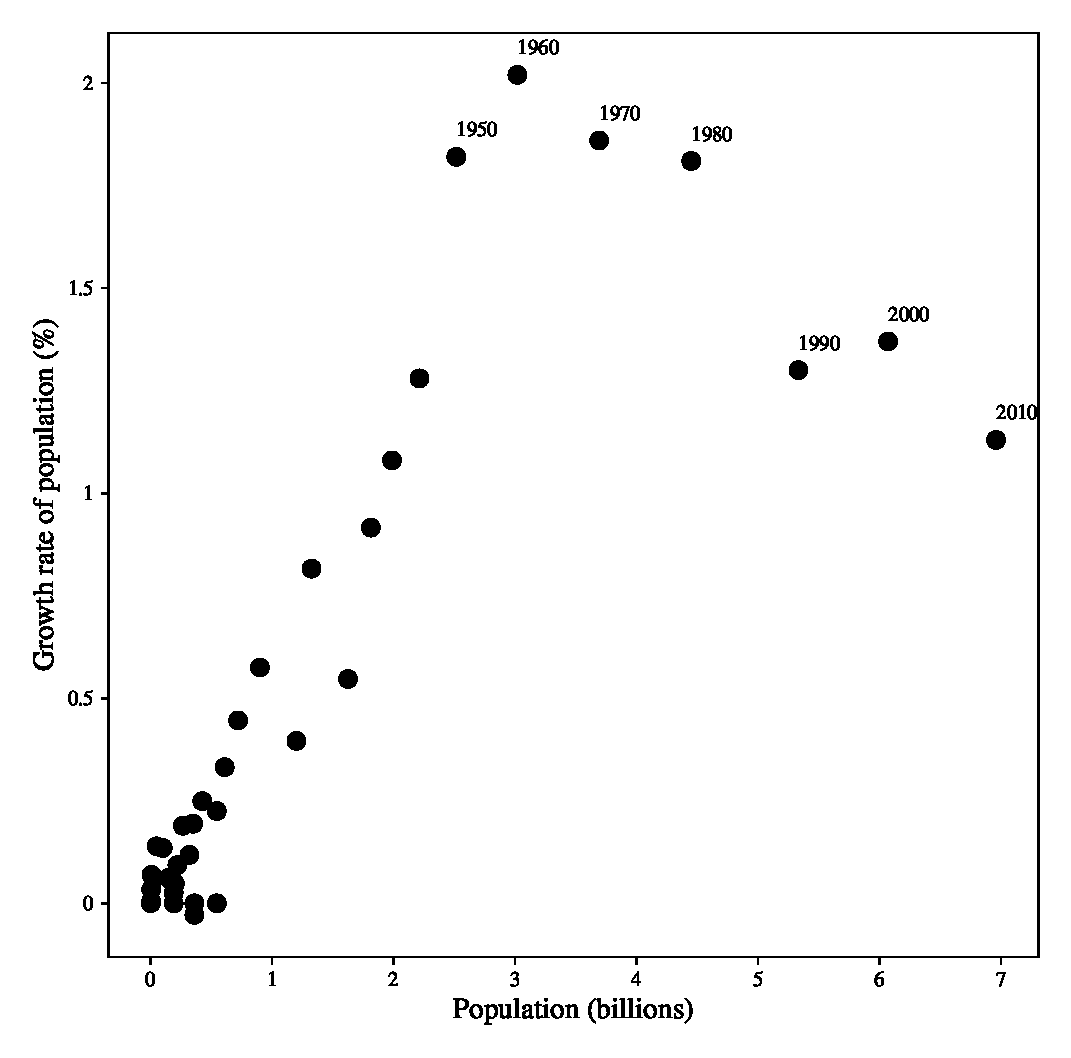
\includegraphics[height=3in]{../Figures/fig-ch9-fig3.eps}
\end{center}
\end{frame}

\section{The transition to growth}
\begin{frame}{Escaping Malthus}
Endogenous technology means that $g_A$ goes up as $L$ goes up. By itself that cannot end Malthusian trap.
\begin{itemize}
	\item $g_A$ keeps raising living standards, yes
	\item But population growth keeps growing
	\item Cannot break the stagnation problem
	\item And population growth cannot, biologically, continually get higher
\end{itemize}
What does a more realistic situation look like?
\end{frame}

\begin{frame}{Realistic function for $g_L$}
\begin{center}
\includegraphics[height=3in]{../Figures/fig-ch9-fig4.eps}
\end{center}
\end{frame}

\begin{frame}{Escaping Malthus}
With realistic population growth function
\begin{itemize}
	\item There is a Malthusian steady state at $y_M^{ss}$. 
	\item If $y(0) < y^{ss}_T$ to begin, will end up in Malthusian state
	\item But if $y_t > Y^{ss}_T$, end up with sustained growth as $g_A > g_L$ always
	\item How did we get past this turning point?
\end{itemize}
\end{frame}

\begin{frame}{The transition to sustained growth}
\begin{center}
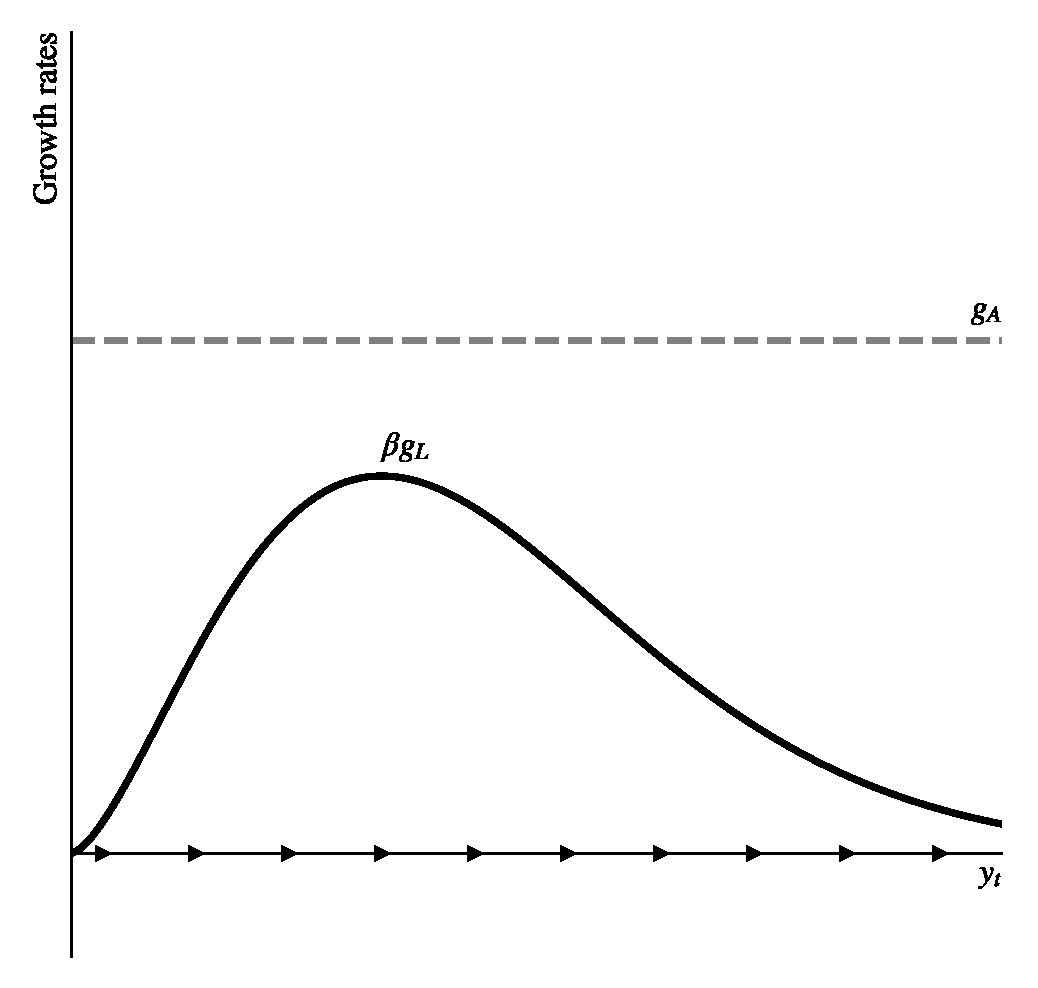
\includegraphics[height=3in]{../Figures/fig-ch9-fig5.eps}
\end{center}
\end{frame}

\begin{frame}{Escaping Malthus}
A reasonable story for the transition to sustained growth:
\begin{itemize}
	\item The world/economy was in/near Malthusian steady state $y_{ss}^M$
	\item But at this steady state $g_L > 0$, so population grew
	\item Because $L$ grew, from endogenous innovation $g_A$ grew
	\item The level of $y_{ss}^M$ grew, so higher $g_L$, etc..
	\item And eventually $g_A$ was high enough that population growth could not keep up
	\item Which allowed growth to continue past the point of $y_{ss}^T$
	\item And entered the world where population growth \textit{falls} with living standards
	\item Which puts us in the world of Solow/Romer/Schumpeter
\end{itemize}
\end{frame}

\section{Comparative development}
\begin{frame}{Early and late escapees}
Some areas escaped Malthus before others:
\begin{itemize}
	\item England is typical example of first industrializing nation around late 1700s (maybe earlier)
	\item But England and Europe were typically far poorer than China or much of Asia historically
	\item What makes sense for earlier take-off in Europe versus Asia?
\end{itemize}
\end{frame}

\begin{frame}{Using the Malthusian model}
The \textit{growth rate} of technology is more important than the \textit{level} of technology:
\begin{itemize}
	\item The escape from Malthus happens when $g_A > g_L$ for a sustained period of time
	\item Asia had large populations, so $g_A$ could be large
	\item But Europe may have had advantage in lower $g_L$ at any given level of living standards?
	\item Or a fortunate burst of innovation, raising $g_A$ even for a few decades, was sufficient to get over the hump
\end{itemize}
\end{frame}

\section{Economics of population growth}
\begin{frame}{Family choice problem}
Population growth is a choice, constrained by resources to have and keep kids alive. Let
\begin{equation}
	U = c^{\gamma}n^{1-\gamma}. \nonumber
\end{equation}
and families care about consumption, $c$, and number of kids $n$. $\gamma$ tells us how much they care about each. Their budget is
\begin{equation}
	y = c + p_n n. \label{EQ_budget_malthus}
\end{equation}
and $p_n$ is the ``cost'' of a child in terms of time, resources, food, etc. There is a trade-off with consumption. 
\end{frame}

\begin{frame}{Utility maximization}
Standard conditions are
\begin{eqnarray}
	MU_c &=& \gamma \frac{U}{c} \nonumber \\ 
	MU_n &=& (1-\gamma) \frac{U}{n}. \nonumber
\end{eqnarray}
and 
\begin{equation}
	\frac{MU_n}{MU_c} = \frac{p_n}{1}, \nonumber
\end{equation}
which can be solved with budget for
\begin{equation}
	n = \frac{(1-\gamma)y}{p_n}. \label{EQ_n_equil}
\end{equation}
Kids/population growth depends positively on income and negatively on their relative cost.
\end{frame}

\begin{frame}{The cost of kids}
Let the cost of children be
\begin{equation}
	p_n = \overline{c}e^{\eta y}. \label{EQ_pn_function}
\end{equation}
\begin{itemize}
	\item There is some subsistence cost, $\overline{c}$
	\item Their cost goes up with income, $y$
	\item Because of the $e^{\eta y}$ the cost is ``convex'' or increases faster as $y$ goes up
	\item This captures that as incomes go up, taking time for kids is more costly (people delay familiy formation)
	\item It also captures that as $y$ goes up you might invest more in kids (school, health) so having more kids gets even more expensive (send 2 kids through college rather than 4 through high school). 
\end{itemize}
\end{frame}

\begin{frame}{Population growth}
Put this together and you have
\begin{equation}
	n = \frac{(1-\gamma)y}{\overline{c}e^{\eta y}}. \nonumber
\end{equation}
\begin{itemize}
	\item Population growth depends in two ways on living standards, $y$
	\item $n$ goes up because of $y$ because families have more resources
	\item $n$ goes down with $y$ because the price of children rises
\end{itemize}
\end{frame}

\begin{frame}{Population growth}
The two effects of $y$ change in how strong they are, leading to
\begin{eqnarray}
	\frac{\partial g_L}{\partial y} &>& 0 \text{ if } y < \frac{1}{\eta} \nonumber \\ 
	\frac{\partial g_L}{\partial y} &=& 0 \text{ if } y = \frac{1}{\eta} \nonumber \\ 
	\frac{\partial g_L}{\partial y} &<& 0 \text{ if } y > \frac{1}{\eta}. \nonumber
\end{eqnarray}
At low levels of $y$, higher $y$ raises population growth. At high levels, higher $y$ lowers population growth. This creates the ``hump'' shape that allows for sustained growth. 
\end{frame}
\end{document}